
\section{CROW: Code Randomization Of WebAssembly}
\label{section:crow}

%\todo{Really bad explanation.}

This section describes CROW \cite{CROW}, our first contribution. Following the workflow in \autoref{diagrams:generic}, CROW is a tool tailored to create semantically equivalent \wasm variants out of LLVM IR passed through the LLVM frontend to be compiled as \wasm code.
In \autoref{diagrams:crow}, we describe the architecture of CROW to create program variants.
The figure highlights the main two components of the Diversifier, \textit{exploration} and \textit{combining}. The workflow starts by passing the input LLVM IR to perform the \emph{exploration}. During the \emph{exploration} process, at the instruction level for each function in the input LLVM IR, CROW produces a collection of functionally equivalent code replacements.  
%In the following, we enunciate the definitions we use along with this work for a code block, functional equivalence, and code replacement. 
In the \emph{combining} stage, CROW assembles the code replacements to generate different LLVM bitcode variants. 
Then, the corresponding backend compiles the LLVM IR variants into \wasm binaries.

In the following, we describe our engineering decisions. All our implementation choices are based on one premise: each implementation decision should increase the number of \wasm variants that CROW creates.
\\
\\
%\subsection*{Overview}

\begin{figure*}[h]
    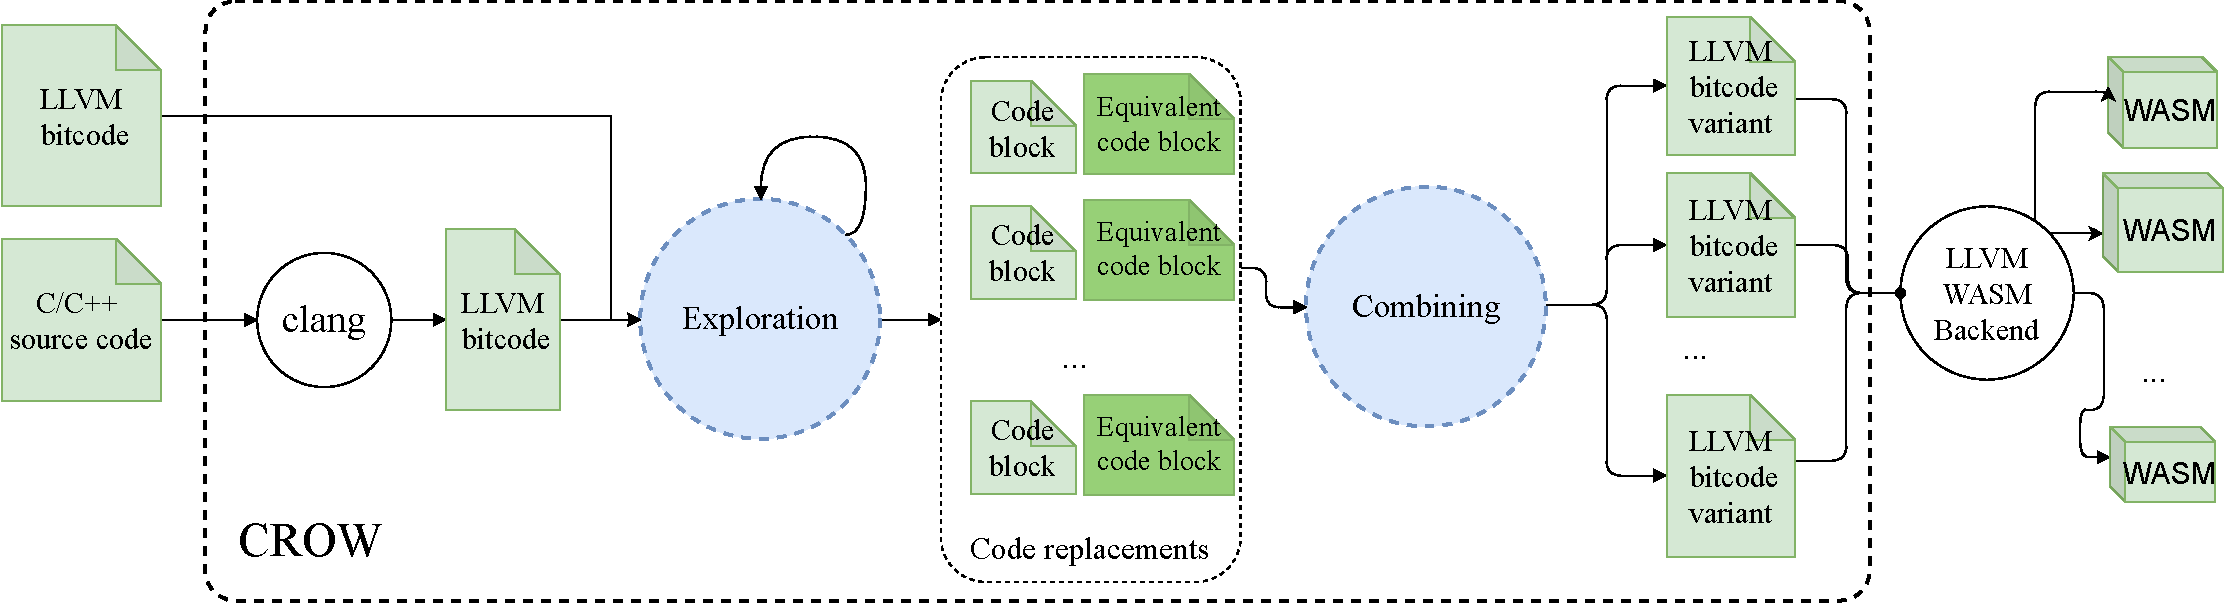
\includegraphics[width=\linewidth]{diagrams/generation/crow.drawio.pdf}
    \caption{CROW components following the diagram in \autoref{diagrams:generic}. CROW takes LLVM bitcodes to generate functionally equivalent code replacements. Then, CROW assembles program variants by combining them.}
    \label{diagrams:crow}
\end{figure*}


%CROW operates at the code block level, taking them from the functions defined inside the input LLVM bitcode module. 
%In addition, the retargeted superoptimizer is in charge of finding the potential places in the original code blocks where a replacement can be applied. Finally, we use the enumerative synthesis strategy of the retargeted superoptimizer to generate code replacements.
%The code replacements generated through synthesis are verified, according to \autoref{def:functional-equivalence}, by internally using a theorem prover. 

\begin{comment}

\begin{definition}{Block (based on Aho \etal \cite{ahodragonbook}):}\label{def:code-block}
    Let $P$ be a program. A block $B$ is a grouping of declarations and statements in $P$ inside a function $F$. 
\end{definition}

\todo{Move to chapter 2}

\begin{definition}{Functional equivalence modulo program state (based on Cohen \etal \cite{cohen1993operating}):}
    \label{def:functional-equivalence}
    Let $B_1$ and $B_2$ be two code blocks according to \autoref{def:code-block}. We consider the program state before the execution of the block, $S_i$, as the input and the program state after the execution of the block, $S_o$, as the output. $B_1$ and $B_2$ are functionally equivalent if given the same input $S_i$ both codes produce the same output $S_o$.
\end{definition}

\begin{definition}{Code replacement:}
    \label{def:code-replacement}
    Let $P$ be a program and $T$ a pair of code blocks $(B_1, B_2)$. $T$ is a candidate code replacement if $B_1$ and $B_2$ are both functionally equivalent as defined in \autoref{def:functional-equivalence}.
    Applying $T$ to $P$ means replacing $B_1$ by $B_2$. The application of $T$ to $P$ produces a program variant $P'$ which consequently is functionally equivalent to $P$.     
\end{definition}
\end{comment}


\subsection{Exploration}

%\subsection*{Variants' generation}

The key component of CROW if its code replacements generation strategy. The diversifier implemented in CROW is based on the work of Jacob \etal \cite{jacob2008superdiversifier}. Their work uses code superoptimization to generate software diversification for x86 with an approach called superdiversification. 
% How a superoptimizer works
Jacob and colleagues cornerstone, code superoptimization, focuses on \emph{searching} for a new program which is faster or smaller than the original code, while preserving its functionality.
The concept of superoptimizing a program dates back to 1987, with the seminal work of Massalin \cite{Massalin1987} which proposes an exhaustive exploration of the solution space. The search space is defined by choosing a subset of the machine's instruction set and generating combinations of optimized programs, sorted by length in ascending order. If any of these programs are found to perform the same function as the source program, the search halts. The main difference between the superoptimization process and a superdiversifier it that the latter keeps all intermediate search results despite their performance. 

% Why and main change
We use the seminal work of Jacob and colleagues to implement CROW because of two main reasons.
First, the code replacements generated by this technique outperform diversification strategies based on hand-written rules. Besides, this technique is fully automatic.
Second, there is a battle tested superoptimizer for LLVM, Souper \cite{Sasnauskas2017Souper:Superoptimizer}. This latter, makes feasible the construction of a generic LLVM superdiversifier.

% This paragraph is hard to read
% How Souper works and why we can modify if
We modify Souper to keep all possible solutions in their searching algorithm. The searching algorithm of Souper is based on inferring the smallest Data Flow Graph for all integer returning instructions in the input LLVM IR. For a given integer returning instruction, it exhaustively builds all possible expressions from a subset of the LLVM IR language.
Each syntactically correct expression in the search space is semantically checked versus the original. The search halts when a semantically equivalent expression is found. Souper synthesizes the replacements in increasing size, thus, the first found equivalent transformation is the best and is the result of the searching. Instead of stopping the process as soon the first equivalent transformation is found, we remove it, keeping more equivalent replacements during the searching. 

Notice that the searching space exponentially increases with the size of the LLVM IR language subset. Thus,
% Additional changes, not needed instructions
we prevent Souper from synthesizing instructions that have no correspondence in the \wasm backend. This decision reduces the searching space. For example, creating expression having the  \texttt{freeze} LLVM instructions will increase the searching space for an instruction without a Wasm  suitable opcode in the end.
% removal or pruning strategies
Moreover, we disable the majority of the pruning strategies of Souper for the sake of more variants. For example, Souper avoids to construct redundant expressions such as commutative operations. We disable strategies like this for the sake of more statically different programs.  %Our modified version of Souper can be found at \todo{}.

%\subsection*{Variant's equivalence}

As we discussed in \autoref{sota:sota}, the equivalence checking is an important part of any program transformation process. In the case of CROW, we quarantee the equivalence property for program variants through Souper as well. Souper uses Z3 \citationneeded, an SMT solver, to check for programs equivalence.  Besides, as a sanity check, it uses KLEE and Alive to double-check that the generated LLVM IR binary out of the code replacement is valid.

% Souper
%Souper is an state-of-the-art superoptimizer for LLVM. It enumerates a set of several optimization candidates to be replaced.
%Souper is based on a Satisfiability Modulo Theories (SMT) solver. SMT solvers are useful for both verification and synthesis of programs \cite{10.1007/978-3-540-78800-3_24}.

%We implement the \emph{exploration} stage of CROW by retargeting Souper. The main objective of Souper is to find the best (smallest) possible program,  

\subsection{Constant inferring}

By extending Souper as a superdiversifier, we contribute with a new mutation strategy, \emph{constant inferring} (in addition to the before mentioned strategies in \autoref{sota:sota}).  
The main component of Souper infers pieces of code as a single constant assignment particularly for boolean valued variables that are used to control branches.
If a program branching is removed due to a constant inferring, the generated program is considerably different to the original program, statically and dynamically.

Let us illustrate the case with an example.
The Babbage problem code in \autoref{babbage} is composed of a loop which stops when it discovers the smaller number that fits with the Babbage condition in Line 4.


{


\begin{minipage}[t]{0.5\linewidth}
        \lstset{
        language=C,
        style=CStyle,
        columns=fullflexible,
        breaklines=true,
        belowcaptionskip=30pt,
        abovecaptionskip=1pt,
        columns=fullflexible,
        breaklines=true, 
        caption={Babbage problem.},
        label=babbage,
        postbreak=\mbox{\textcolor{red}{$\hookrightarrow$}\space}
    } 
    \begin{lstlisting}[numbers=left]
    int babbage() {
        int current = 0,
            square;
        while ((square=current*current) % 1000000 != 269696) {
            current++;
        }
        printf ("The number is %d\n", current);
        return 0 ;
    }
    \end{lstlisting}
\end{minipage}
\begin{minipage}[t]{0.5\linewidth}
        \lstset{
        language=C,
        style=CStyle,
        columns=fullflexible,
        breaklines=true,
        belowcaptionskip=3pt,
        abovecaptionskip=1pt,
        columns=fullflexible,
        breaklines=true, 
        caption={Constant inferring transformation over the original Babbage problem in \autoref{babbage}.},
        label=inferring,
        postbreak=\mbox{\textcolor{red}{$\hookrightarrow$}\space}
    } 
    \begin{lstlisting}[]
int babbage() {
    @int current = 25264;@
    
    


    printf ("The number is %d\n", current);
    return 0 ;
}
    \end{lstlisting}
\end{minipage}
}
% llvm-opt: rool unroll
In theory, this value can also be inferred by unrolling the loop the correct number of times with the LLVM toolchain.
However, standard LLVM tools cannot unroll the \texttt{\textbf{while}}-loop because the loop count is too large.
% Souper
Souper can deal with this case, generating the program in \autoref{inferring}. It infers the value of \texttt{current} in Line 2 such that the Babbage condition is reached. Therefore, the condition in the loop will always be false. Then, the loop is dead code, and is removed in the final compilation. It is clear that the new program in \autoref{inferring} is remarkably smaller and faster than the original code. Notice that for the sake of illustration, we show both codes in C language, this process inside CROW is performed directly in LLVM IR. Also notice that the two programs in the example follow the definition of \emph{functional equivalence} discussed in \autoref{sota:sota}.

\subsection{Combining replacements}

When we retarget Souper, to create variants, we recombine all code replacements, including those for which a constant inferring was performed.
This allows us to create variants that are also better than the original program in terms of size and performance. Most of the Artificial Software Diversification  works generate variants that are as performant or iller than the original program. By using a superdiversifier, we could be able to generate variants that are better, in terms of performance, than the original program. This will give the option to developers to decide between performance and diversification without sacrificing the former. 

On the other hand, when Souper finds a replacement, it is applied to all equal instructions in the original LLVM binary. In our implementation, we apply the transformation only to the instruction for which it was found in the first place. For example, if we find a replacement that is suitable for $N$ difference places in the original program, we generate $N$ different programs by applying the transformation in only one place at a time. Notice that this strategy provides a combinatorial explosion of program variants as soon as the number of replacements increases.

\subsection{Removing latter optimizations for LLVM}

During the implementation of CROW we have the premise of removing all builtin optimizations in the LLVM backend that could reverse Wasm  variants.
Therefore, in addition to the extension of Souper, we modify the LLVM compiler and the \wasm backend.
We disable all optimizations in the \wasm backend that could reverse the superoptimizer transformations, such as constant folding and instructions normalization.


%\todo{We disable cost restrictions and the LLVM backend optimizations...maybe for the assesment RQ ?}


